\documentclass[12pt]{article}
\usepackage{graphicx} % Required for inserting images
\usepackage{hyperref}
\usepackage[margin=1.27cm]{geometry}
\usepackage{mathptmx, newtxmath}
\usepackage{amsmath}
\usepackage{indentfirst}
\setlength{\parindent}{2em}

\title{Report: MA6217 Problem-Based Assignment 1}
\author{Yang Jiaxin, Matriculation No.: G2605405J}
\date{5/9/2026}

\begin{document}

\maketitle

Check all the codes, Simulink files, images, raw data and report at ntulearn or:

\href{https://github.com/MrOxOrOxen/ntu/tree/ma6217/PBA1}{github.com/MrOxOrOxen/ntu/tree/ma6217/PBA1}.

\section{Task 1}

\subsection{Overall system architecture}

Figure \ref{fig:overall} shows the architecture of the overall top-level system in Simulink.

\begin{figure}[h]
    \centering
    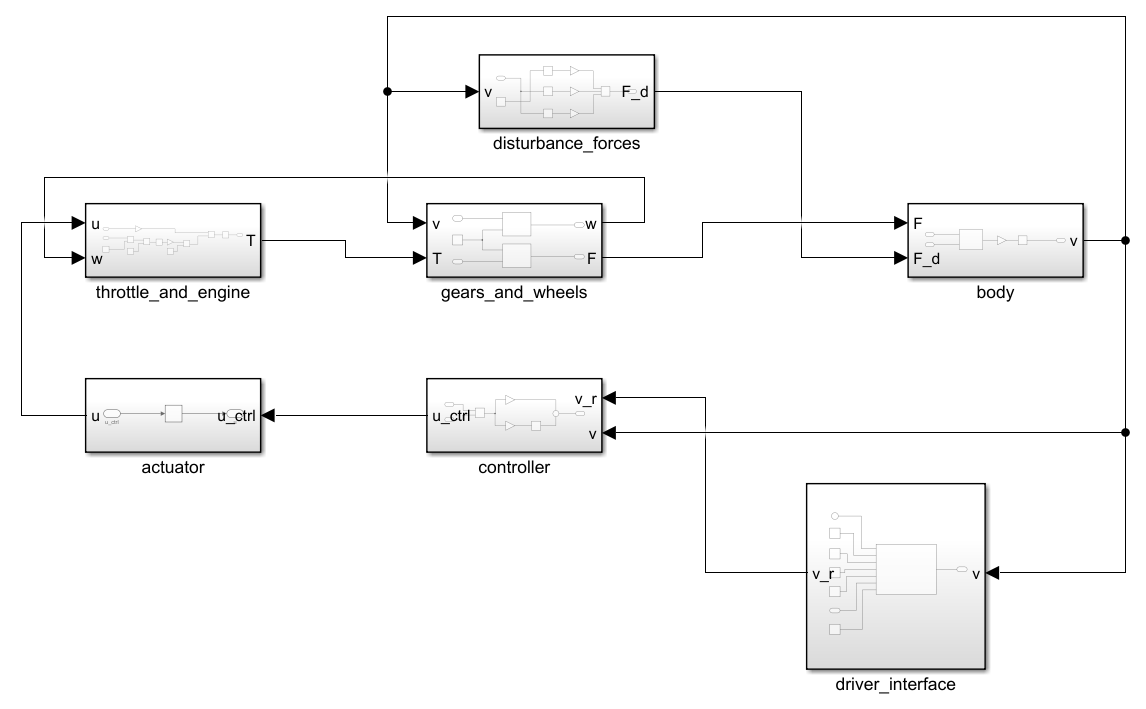
\includegraphics[width=0.9\linewidth]{src/figure1.png}
    \caption{Overall system architecture}
    \label{fig:overall}
\end{figure}

Table \ref{tab:physical_quantities} shows the meanings of the physical quantities shown in figure \ref{fig:overall}.

\begin{table}[htbp]
    \centering
    \begin{tabular}{ccc}
    \hline
        Physical Quantity & Meaning & Unit \\
    \hline
        $u_{ctrl}$ & Ideal throttle signal & / \\
        $u$ & Actual throttle position & / \\
        $\omega$ & Engine rotational speed & $rad/s$ \\
        $T$ & Engine torque & $N\cdot m$ \\
        $v$ & Actual vehicle speed & $m/s$ \\
        $v_r$ & Target vehicle speed & $m/s$ \\
        $F$ & Engine traction force & $N$ \\
        $F_d$ & Disturbance force & $N$ \\
    \hline
    \end{tabular}
    \caption{Physical Quantities in overall structure}
    \label{tab:physical_quantities}
\end{table}

As illustrated in Figure \ref{fig:overall}, the overall model operates as a closed-loop control system. The overall signal paths flow as follows:

- \textit{Driver interface}: Generate the target speed $v_r$ from the user input (cruise control signal) and the real-time vehicle speed $v$.

- \textit{Controller}: Input target speed $v_r$ and real-time speed $v$, compute tracking error, and generate the control signal $u_{ctrl}$.

- \textit{Actuator}: Translate $u_{ctrl}$ into the actual throttle position $u$.

- \textit{Throttle and Engine}: Input the throttle position $u$ and engine rotational speed $\omega$, and calculate engine torque $T$.

- \textit{Gears and wheels}: Receive engine torque $T$ and vehicle speed $v$, and convert them to traction force $F$ while back-calculating the engine rotational speed $\omega$ based on the selected gear ratio $\alpha_n$.

- \textit{Disturbance forces}: Calculate external resistance forces $F_d$ based on the vehicle speed $v$.

- \textit{Body}: Input the traction force $F$ and disturbance force $F_d$, and computes the acceleration and integrates it to vehicle speed $v$.

The details of the subsystems are as follows.

\subsection{Driver Interface}

Figure \ref{fig:driver_interface} shows the structure of the subsystem \textit{Driver interface}, where \textit{clock} is the simulation time (will be used in the following tasks), and the other inputs are loaded from the file \textit{constants.m}.

\begin{figure}[htbp]
    \centering
    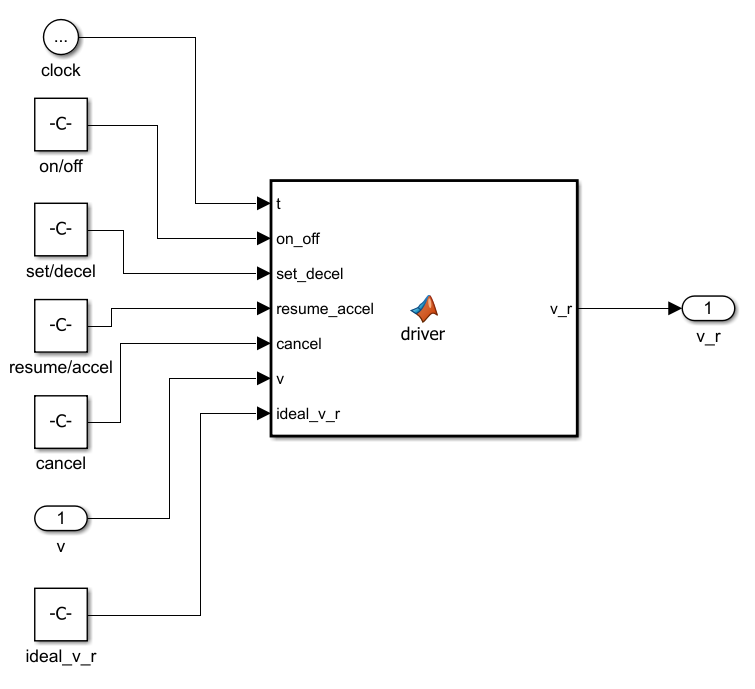
\includegraphics[width=0.7\linewidth]{src/figure2.png}
    \caption{Structure of Subsystem \textit{Driver Interface}}
    \label{fig:driver_interface}
\end{figure}

The \textit{driver} MATLAB function models driver interaction with the cruise control system, in which persistent variables $target\_v$ and $is\_active$ maintain system state memory access execution time steps. The subsystem logic handles five distinct operational conditions:

1. System disablement ($on\_off = 0$): Deactivates cruise control ($is\_active = false$) and directly passes through the current vehicle speed $v$ to $v_r$.

2. Cruise cancellation ($cancel = 1$): The same as above, but can store the current speed $v$ in the variable $target\_v$ for future resumption.

3. Target speed set ($set\_decel = 1$): Activates cruise mode ($is\_active = true$) and latches $ideal\_v\_r$ as the new setpoint velocity $target\_v$.

4. Speed increment ($resume\_accel = 1$):

- If cruise control is active, it increase the current setpoint by 1 m/s in each sampling time (i.e. 0.01 s in my setting).

- If inactive, it re-activates the cruise at $target\_v$.

5. Output multiplexing: When $is\_active$ is \textit{true}, the function outputs the latched $target\_v$. Otherwise, it outputs the actual vehicle speed $v$.

The conditions mean that if cruise is activated, the goal speed will be the speed that the driver sets manually; otherwise, the goal speed will be the actual speed of the vehicle.

Set the sampling time of MATLAB function as 0.01 s rather than -1 to prevent runtime error.

\subsection{Controller}

Figure \ref{fig:controller} shows the structure of the subsystem \textit{Controller}, where $k_i$ and $k_p$ are self-defined in the file \textit{constants.m}.

\begin{figure}[htbp]
    \centering
    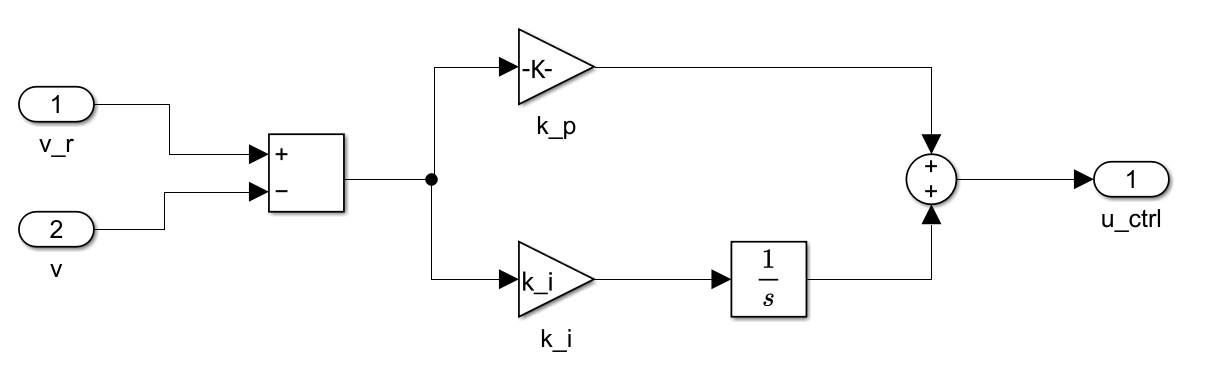
\includegraphics[width=0.8\linewidth]{src/figure3.png}
    \caption{Structure of Subsystem \textit{Controller}}
    \label{fig:controller}
\end{figure}

The controller follows the PI control equation:

\begin{equation}
    u(t) = k_p e(t) + k_i \int_0^t e(\tau)d\tau
    \label{eq:pi}
\end{equation}

where $e(t) = v_r - v$ is the system tracking error. Initial conditions of the integrator vary according to the requirements of different tasks.

\subsection{Actuator}

Figure \ref{fig:actuator} shows the structure of the subsystem \textit{Actuator}. The saturation block is used to limit the maximum and minimum value of the input $u_{ctrl}$, i.e.

\begin{equation}
    u(t) = 
    \begin{cases}
    1, & u_{ctrl}(t) > 1 \\
    0, & u_{ctrl}(t) < 0 \\
    u_{ctrl}(t), & else \\
    \end{cases}
    \label{eq:ut}
\end{equation}

\begin{figure}[htbp]
    \centering
    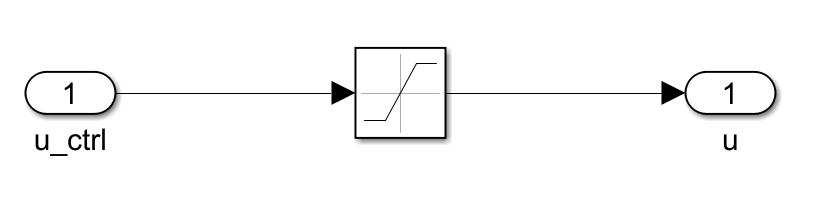
\includegraphics[width=0.6\linewidth]{src/figure4.png}
    \caption{Structure of Subsystem \textit{Actuator}}
    \label{fig:actuator}
\end{figure}

For most of the times, $u$ is larger than 1, so the output is mostly 1.

\subsection{Throttle and engine}

Figure \ref{fig:throttle_and_engine} shows the structure of the subsystem \textit{Throttle and engine}, where:

- The \textit{gain} block after the input $u$ has a gain $T_m$.

- The \textit{gain} block after the square block has a gain $\beta$.

- The variables $\omega_m, \beta$ and $T_m$ come from the file \textit{constants.m}.

There is a saturation block before the output $T$ to make sure $T \ge 0$.

\begin{figure}[htbp]
    \centering
    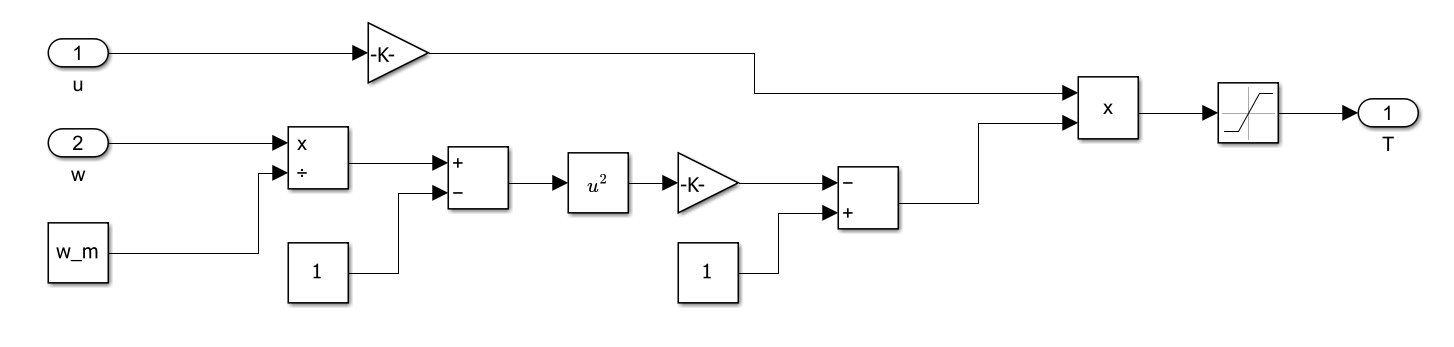
\includegraphics[width=0.8\linewidth]{src/figure5.png}
    \caption{Structure of Subsystem \textit{Throttle and engine}}
    \label{fig:throttle_and_engine}
\end{figure}

The subsystem follows the following equation:

\begin{equation}
    T(\omega, u) = u \cdot T_m [1 - \beta (\frac{\omega}{\omega_m} - 1)^2]
    \label{eq:throttle}
\end{equation}

\subsection{Gears and wheels}

Figure \ref{fig:gears_and_wheels} shows the structure of the subsystem \textit{Gears and wheels}, where the constant block \textit{alpha for task 1-3} is the variable value of $\alpha_1$ to $\alpha_5$ in the file \textit{constants.m}, and the constant block will be replaced by a stateflow chart in task 4.

Change the value of the constant block to simulate the variable gear selection ratios $\alpha_n$ in tasks 1, 2 and 3.

\begin{figure}[htbp]
    \centering
    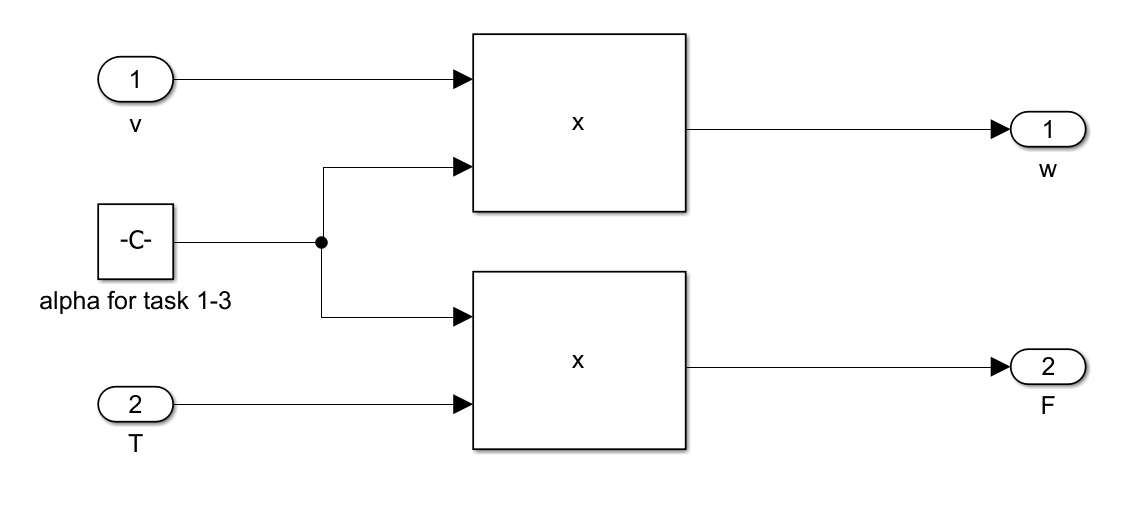
\includegraphics[width=0.7\linewidth]{src/figure6.png}
    \caption{Structure of Subsystem \textit{Gears and wheels}}
    \label{fig:gears_and_wheels}
\end{figure}

The subsystem follows the following equations:

\begin{gather}
    \omega = \alpha_n v
    \label{eq:w=av} \\
    F = \alpha_n T
    \label{eq:F=aT}
\end{gather}

where $n \in \{1, 2, 3, 4, 5\}$.

\subsection{Disturbance forces}

Figure \ref{fig:disturbance_forces} shows the structure of the subsystem \textit{Disturbance forces}, where:

- The \textit{gain} block after the sine block has a gain of $m\cdot g$.

- The \textit{gain} block after the sign block has a gain of $m \cdot g \cdot C_r$.

- The \textit{gain} block after the square block has a gain of $\frac{1}{2}\rho \cdot C_d \cdot A$.

- The variables $\theta, m, g, C_r, C_d, \rho$ and $A$ come from the file \textit{constants.m}.

\begin{figure}[htbp]
    \centering
    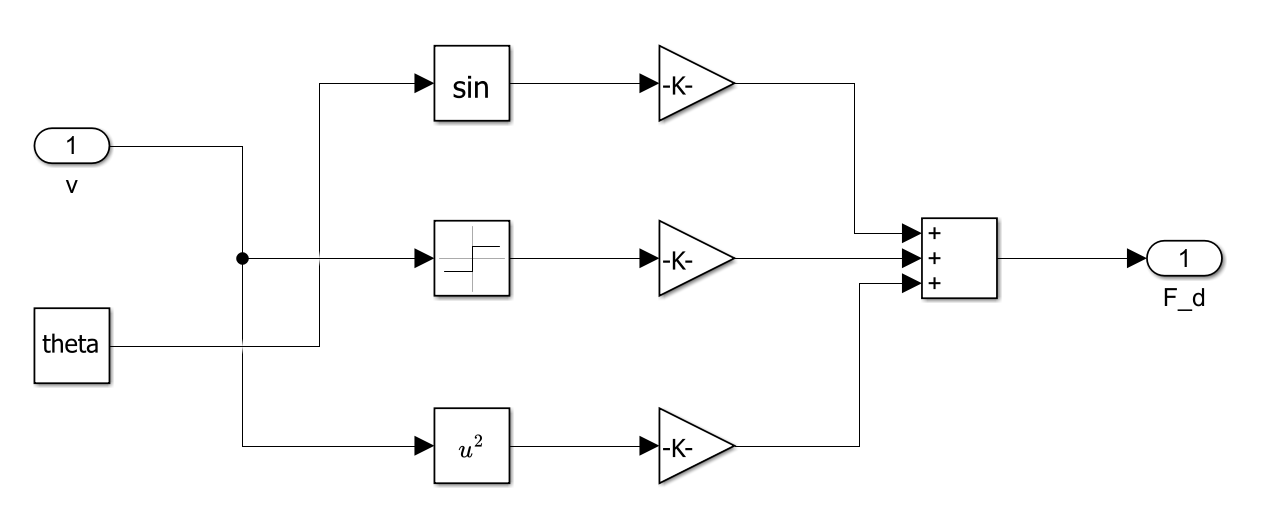
\includegraphics[width=0.8\linewidth]{src/figure7.png}
    \caption{Structure of Subsystem \textit{Disturbance forces}}
    \label{fig:disturbance_forces}
\end{figure}

The subsystem follows the following equation:

\begin{equation}
    F_d = mg\sin\theta + mgC_rsgn(v) + \frac{1}{2}\rho C_d A v^2
    \label{eq:fraction}
\end{equation}

\subsection{Body}

Figure \ref{fig:body} shows the structure of the subsystem \textit{Body}, where the \textit{gain} block after the minus block has a gain of $\frac{1}{m}$, and $m$ comes from the file \textit{constants.m}.

\begin{figure}[htbp]
    \centering
    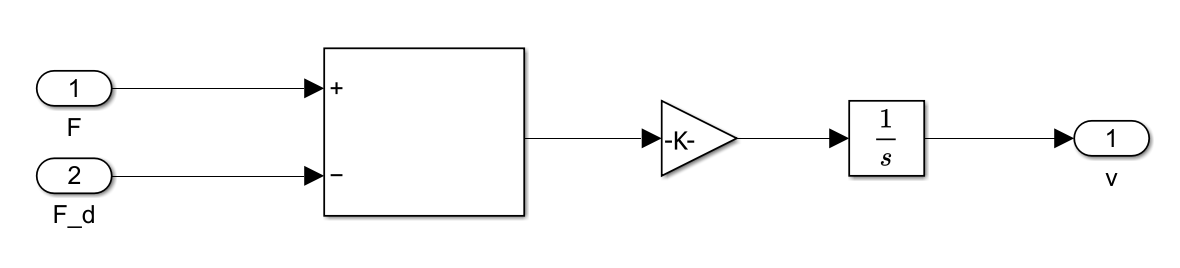
\includegraphics[width=0.8\linewidth]{src/figure8.png}
    \caption{Structure of Subsystem \textit{Body}}
    \label{fig:body}
\end{figure}

The subsystem follows the following equation:

\begin{equation}
    m \frac{dv}{dt} = F - F_d
    \label{eq:newton_2nd_law_eq1}
\end{equation}

i.e.

\begin{equation}
    v(t) = \int_0^t \frac{dv}{d\tau} d\tau = \int_0^t \frac{1}{m} [F(\tau) - F_d(\tau)]
    \label{eq:newton_2nd_law_eq2}
\end{equation}

Initial conditions of the integrator vary according to the requirements of different tasks.

\section{Task 2}

Since task 2 is open-loop and owns a constant value of input $u$, we cut the $u$ connection of subsystem \textit{Actuator} and \textit{Throttle and engine}, and add a constant block to represent $u$ instead. Figure \ref{fig:task2_overall} shows the new overall figure, where the subsystem \textit{Throttle and engine} receives the constant input $u$.

\begin{figure}[htbp]
    \centering
    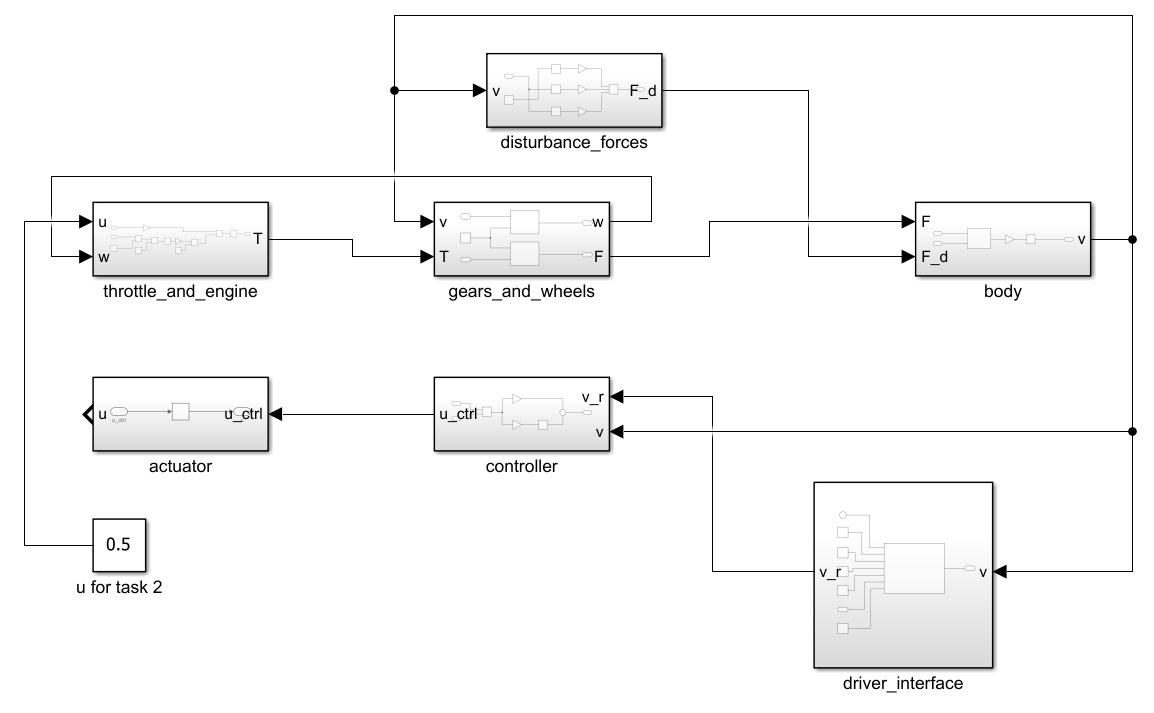
\includegraphics[width=0.9\linewidth]{src/figure9.png}
    \caption{Overall system architecture in Task 2}
    \label{fig:task2_overall}
\end{figure}

\subsection{Simulation Conditions}

\textbf{The initial condition of the integrator (which is defined as the output of the integrator in Simulink):}

- In subsystem \textit{Body}: 0, since the initial velocity of the vehicle is 0.

- In subsystem \textit{Controller}: Any value, since the whole system is open-loop and the \textit{Controller} block is after the output $v$. The initial value of the integrator does not affect the output $v$.

Similarly, the initial value of the self-defined variables ($k_p, k_i, v_r$) doesn't affect the output value $v$. We can set them as any values.

Hence, Table \ref{tab:task2_simcondition} shows the simulation conditions as follows.

\begin{table}[htbp]
    \centering
    \begin{tabular}{cccc}
       \hline
       Parameter & Variable & Value & Unit \\
       \hline
       Gear & / & 1 & / \\
       Transmission ratio & $\alpha_n (\alpha_1)$ & 40 & $rad/m$\\
       Throttle position & $u$ & 0.5 & / \\
       Road slope & $\theta$ & 0 & $deg$ \\ 
       Initial speed (integrator initial condition) & $v(0)$ & 0 & m/s \\
       Goal speed & $v_r$ & any & m/s \\
       Proportion Coefficient & $k_p$ & any & / \\
       Integral Coefficient & $k_i$ & any & / \\
       Output & $v$ & / & m/s \\
    \hline
    \end{tabular}
    \caption{Simulation Conditions in Task 2}
    \label{tab:task2_simcondition}
\end{table}

\subsection{Result}

Figure \ref{fig:task2_result} shows the velocity-time image of the open-loop control in task 2. 

It is clear that the vehicle accelerates from the start, but stables at a certain velocity after a period of time, since the disturbance force increases with the increase of speed $v$ according to equation \ref{eq:fraction}, and according to equation \ref{eq:newton_2nd_law_eq1} and \ref{eq:newton_2nd_law_eq2}, the acceleration will be 0 because $F - F_d = 0$, and there is no velocity increase then.

\begin{figure}[htbp]
    \centering
    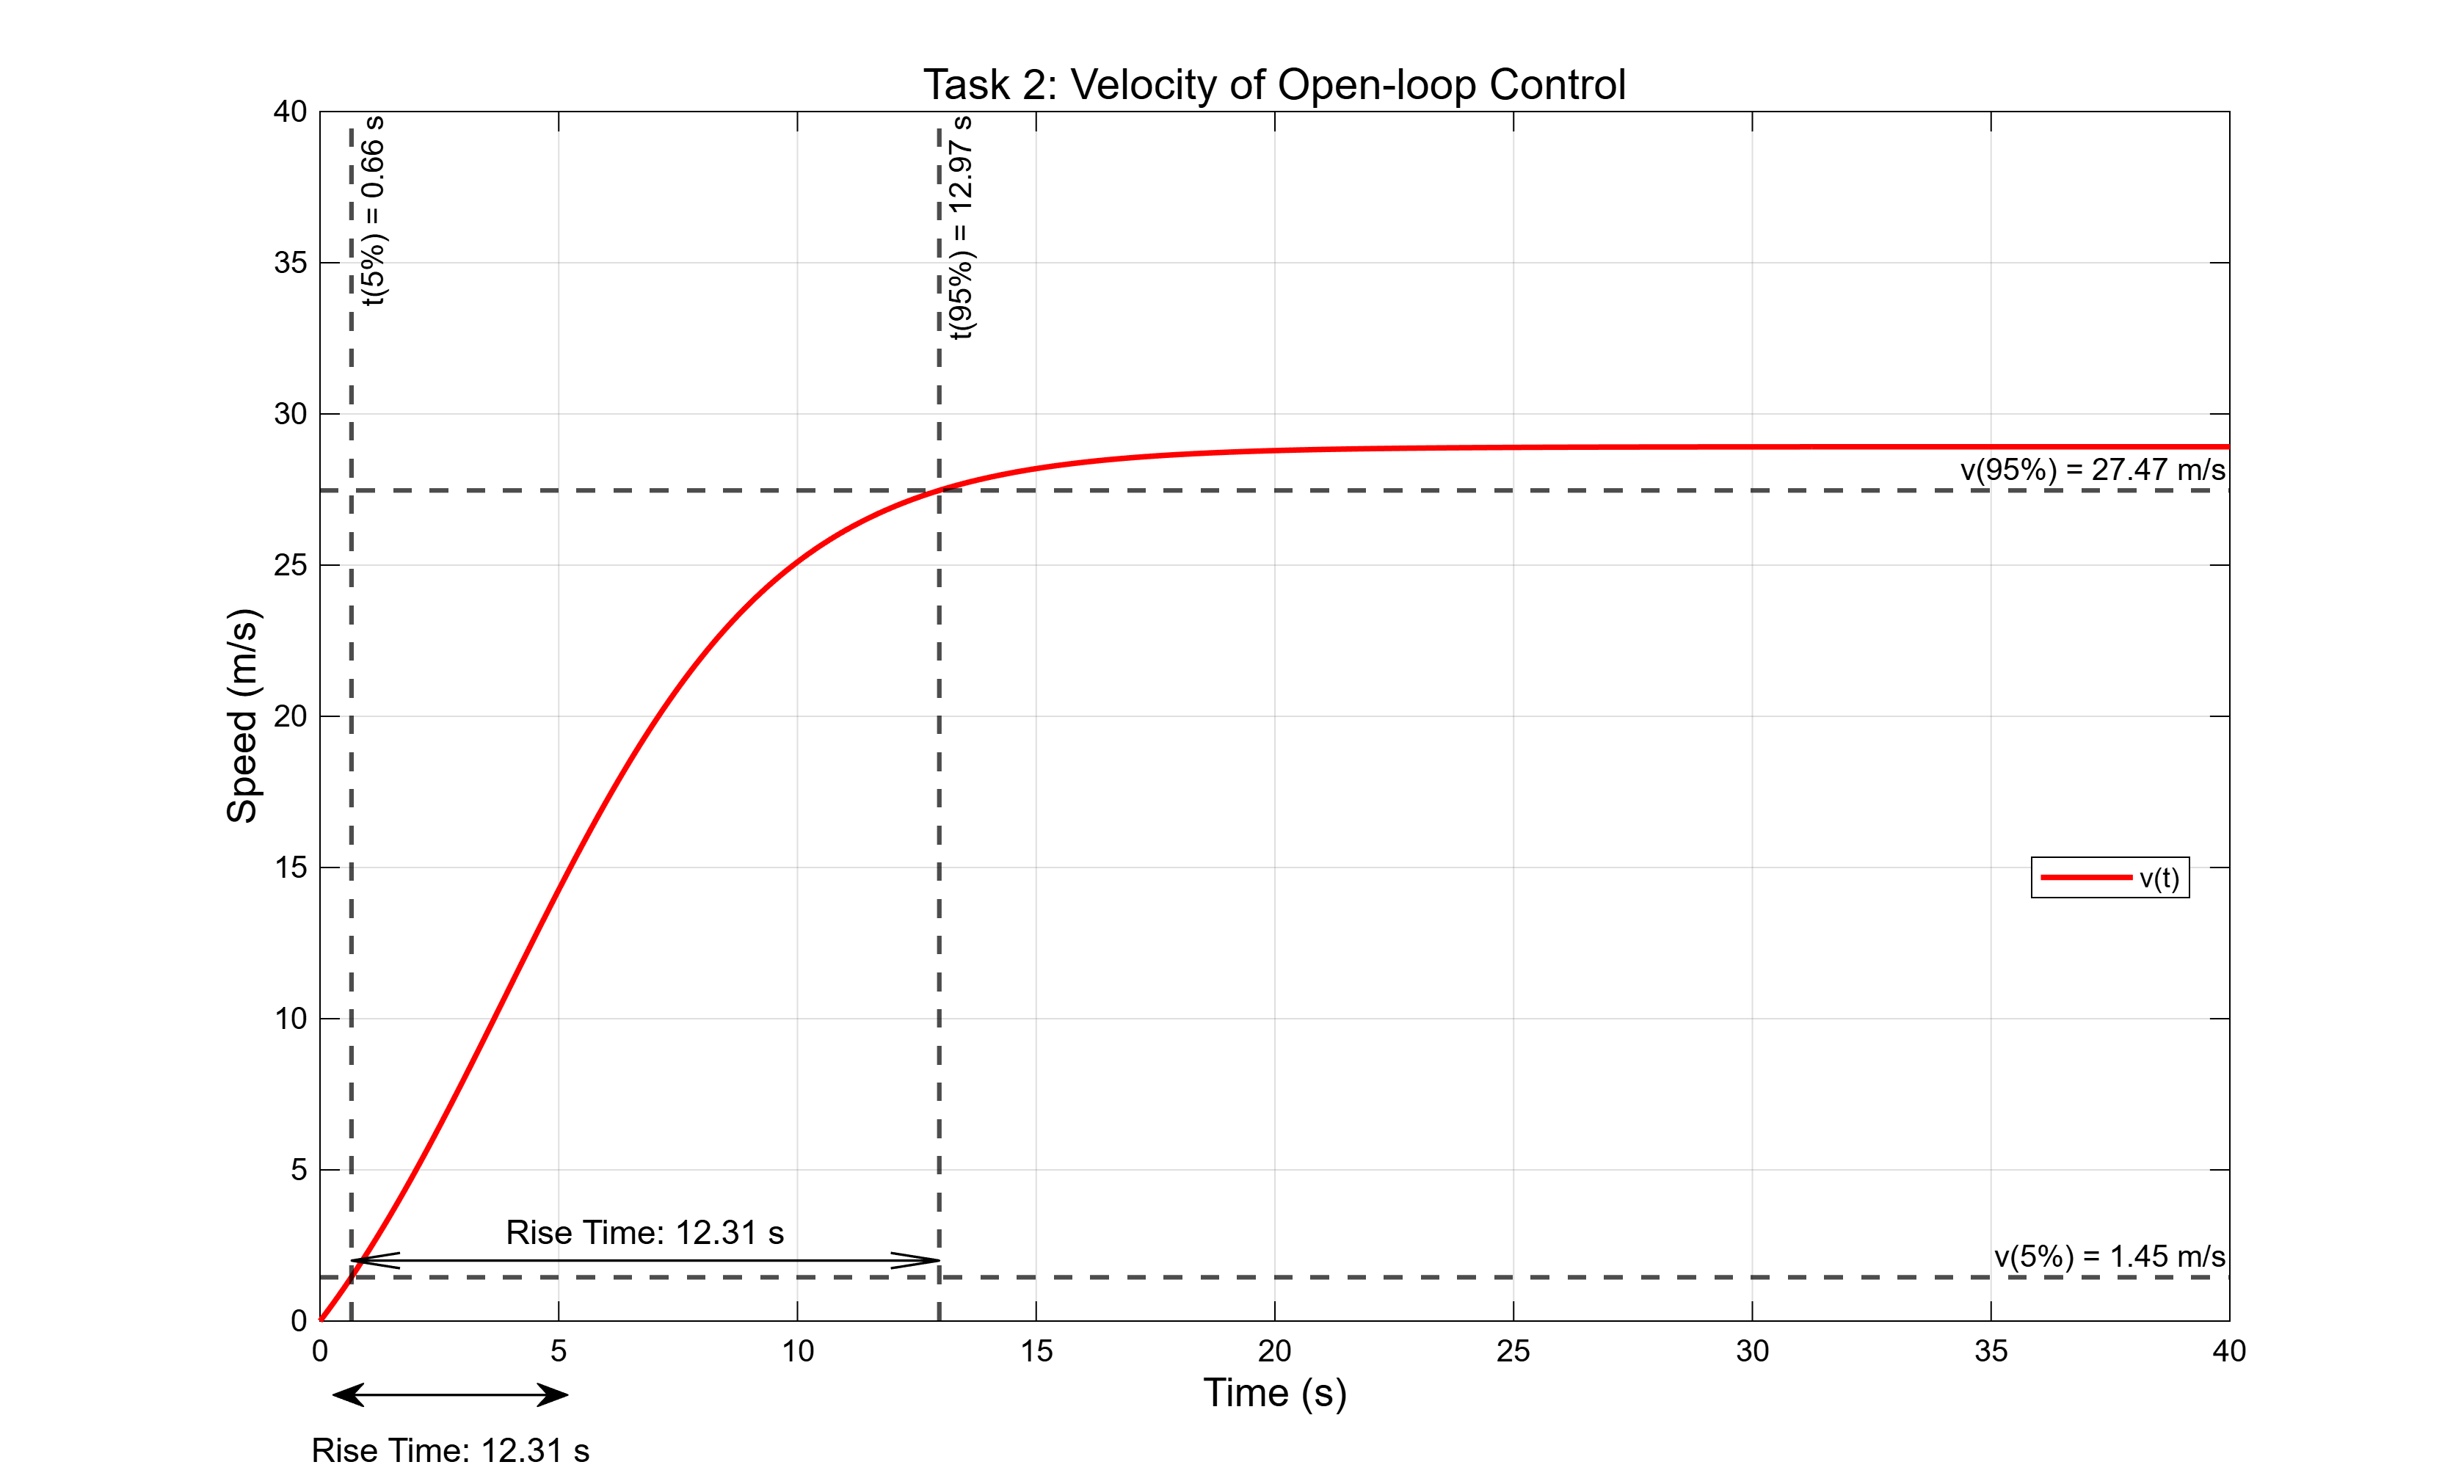
\includegraphics[width=1\linewidth]{src/task2.png}
    \caption{Velocity of open-loop control in Task 2}
    \label{fig:task2_result}
\end{figure}

Actually, I set the simulation time as 100 s, and Figure \ref{fig:task2_result} only shows the result in the first 40 seconds. According to the raw data, the output $v$ is stable when the time approaches 100 s.

Hence, we can consider that the mean speed over the final 5\% of the simulation (i.e. 95 - 100 s) can be regarded as the steady-state speed. And by the way, by calculating the mean speed of the last 5 seconds, we can define how accurately the final speed matches the target speed.

According to the raw data and code execution result, the simulation results are as follows:

\begin{table}[htbp]
    \centering
    \begin{tabular}{cc}
    \hline
        Initial speed & 0 m/s \\
        Vehicle speed at the end of $t$ & 28.9151 m/s \\
        Steady-state speed & 28.9151 m/s \\
        5\% of steady-state speed & 1.4458 m/s \\
        95\% of steady-state speed & 27.4693 m/s \\
        Time for 5\% speed & 0.66 s \\
        Time for 95 \% speed & 12.97 s \\
        Rise time & 12.31 s \\
    \hline
    \end{tabular}
    \caption{Simulation Result of Task 2}
    \label{tab:task2_simresult}
\end{table}

\section{Task 3}

Task 3 is a closed-loop task, so its top-level simulation architecture is the same as Figure \ref{fig:overall}, but with a different input $\alpha_3 = 16$.

\subsection{Simulation Conditions}

\textbf{The initial condition of the integrator (the output of the integrator at $t=0^+$):}

- In subsystem \textit{Body}: 20, since the initial velocity of the vehicle is 20 m/s.

- In subsystem \textit{Controller}: 0.1042, whose steps of calculating is as follows.

Since task 3 asks us to maintain the vehicle velocity $v$ at 20 m/s for a period of time, we need to ensure the acceleration $a$ of the vehicle at $v=20m/s$ is 0, which is:

\begin{gather}
    F - F_d = 0
    \label{eq:task3_eq_newton} \\
    F = F_d = mg\sin\theta + mgC_rsgn(v) + \frac{1}{2}\rho C_d A v^2 = 323.64 N \cdot m
    \label{eq:task3_eq_friction} \\
    T = \frac{F}{\alpha_3} \approx 20.2275 N \cdot m
    \label{eq:task3_eq_torque}
\end{gather}

And then reverse calculate the throttle position $u$ to maintain the steady state:

\begin{gather}
    \omega = \alpha_3 v = 320 rad/s
    \label{eq:task3_omega} \\
    u(0) = \frac{T}{T_m[1-\beta(\frac{\omega}{\omega_m}-1)^2]} \approx 0.1042
    \label{eq:task3_u}
\end{gather}

When $t=0$, the tracking error $e(0) = v_d(0) - v(0)$ should be 0 since $v_d(0) = v(0)$.

Define the output value of the integrator as $x(t)$. According to the equation of PI controller (function \ref{eq:pi}) and my Simulink structure:

\begin{equation}
    x(0) = u(0) - k_pe(0) = u(0) \approx 0.1042
    \label{eq:task3_x0}
\end{equation}

which means the initial output of the integrator in \textit{Controller} should be 0.1042.

\textbf{For the goal speed $v_r$:}

In the subsystem \textit{Driver Interface}, set the variable $set\_decel = 1$, which means the cruise has been activated. Set the variable $ideal\_v\_r = 20$ at the beginning of the simulation, and when $t=10s$, set $ideal\_v\_r = 30$, and thus a step increase of the goal speed has been made.

\textbf{For other self-defined variables:}

There are only $k_p$ and $k_i$ left. The adjustment of the two variables will be discussed in the following subsection.

All of the initial conditions are summarized in the table below.

\begin{table}[htbp]
    \centering
    \begin{tabular}{cccc}
       \hline
       Parameter & Variable & Value & Unit \\
       \hline
       Gear & / & 3 & / \\
       Transmission ratio & $\alpha_n (\alpha_1)$ & 16 & $rad/m$\\
       Road slope & $\theta$ & 0 & $deg$ \\ 
       Initial speed (integrator initial condition) & $v(0)$ & 20 & m/s \\
       Goal speed & $v_r$ & 20 & m/s \\
       Proportion Coefficient & $k_p$ & 0.1 & / \\
       Integral Coefficient & $k_i$ & 0 & / \\
       Output & $v$ & / & m/s \\
    \hline
    \end{tabular}
    \caption{Initial Simulation Conditions in Task 3}
    \label{tab:task3_simcondition}
\end{table}

\subsection{Adjustment of PI Control Parameters}

Table \ref{tab:pid} and figure \ref{fig:pid} shows the adjustment of $k_p$ and $k_i$ of the whole system according to the system response.

Specific adjustment process:

\textbf{Step 1 (Row 1 to 4):} In this step, we fix $k_i = 0$ and adjust the value of $k_p$, and find that no matter how large $k_p$ is, the steady-state speed cannot reach our goal speed 30 m/s, and that if $k_p$ is too large, the throttle reaction is extremely sharp. Thus, we choose $k_p=0.2$ where the rise time (can be regarded as reaction time) is suitable and the throttle doesn't react so sharply.

\textbf{Step 2 (Row 5 to 10):} In this step, we fine-tune the value of $k_i$. We firstly make $k_i=0.1$ as the reference value, and notice the 2\% settling time is too long, and that if we increase $k_i$, the settling time is even bigger, so we will decrease $k_i$. Finally we get $k_i=0.006$ where the overshoot, rise time and settling time are suitable.

\textbf{Step 3 (Row 11 to the end):} Fine-tune the value of $k_p$. And thus we get the final values: $k_p=0.24, k_i=0.006$.

\begin{table}[htbp]
    \centering
    \begin{tabular}{cccccccc}
    \hline
       $k_p$ & $k_i$ & Steady Speed & Max Speed & Overshoot & Rise Time & 5\% Settling Time & 2\% Settling Time \\
        &  & (m/s) & (m/s) & (\%) & (s) & (s) & (s) \\
    \hline
        0.1 & 0 & 29.2908 & 29.2908 & / & 10.17 & / & / \\
        0.2 & 0 & 29.6290 & 29.6290 & / & 6.03 & / & / \\
        1 & 0 & 29.9229 & 29.9229 & / & 3.96 & / & / \\
        100 & 0 & 29.9992 & 29.9992 & / & 3.95 & / & / \\
        0.2 & 0.01 & 30.0125 & 30.6198 & 2.0659 & 4.90 & 4.01 & 12.83 \\
        0.2 & 0.015 & 30.0018 & 30.9999 & 3.3329 & 4.47 & 3.85 & 18.04 \\
        0.2 & 0.005 & 30.0319 & 30.1900 & 0.6318 & 5.74 & 4.26 & 5.63 \\
        0.2 & 0.0075 & 30.0248 & 30.4130 & 1.3768 & 5.24 & 4.12 & 5.23 \\
        0.2 & 0.007 & 30.0274 & 30.3699 & 1.2329 & 5.33 & 4.15 & 5.30 \\
        0.2 & 0.006 & 30.0315 & 30.2813 & 0.9378 & 5.52 & 4.20 & 5.45 \\
        0.21 & 0.006 & 30.0330 & 30.2654 & 0.8848 & 5.41 & 4.14 & 5.35 \\
        0.22 & 0.006 & 30.0342 & 30.2518 & 0.8394 & 5.32 & 4.09 & 5.26 \\
        0.23 & 0.006 & 30.0353 & 30.2392 & 0.7973 & 5.23 & 4.04 & 5.17 \\
        0.24 & 0.006 & 30.0363 & 30.2278 & 0.7954 & 5.15 & 4.00 & 5.10 \\
    \hline
    \end{tabular}
    \caption{System Response of Different $k_p$ and $k_i$ Parameters}
    \label{tab:pid}
\end{table}

\begin{figure}[htbp]
    \centering
    \includegraphics[width=1\linewidth]{src/merged.jpg}
    \caption{System Response of Different $k_p$ and $k_i$ Parameters (Enlarge to view)}
    \label{fig:pid}
\end{figure}

\section{Task 4}

There are 3 changes to the overall system:

1. Task 4 is an open-loop system (although for $w$ it is close-loop), so we cut the $u$ connection of the subsystem \textit{Actuator} and \textit{Throttle and Engine}, and add a constant block to represent $u$ signal. 

2. For the gear shifting simulation, we add a stateflow chart (whose input is $\omega$ and output is gear and $\alpha$) to simulate the gear shifting.

3. Since $\alpha$ is an input of the subsystem \textit{Gears and wheels}, we removed the constant block in this subsystem (see Figure \ref{fig:gears_and_wheels}).

Figure \ref{fig:task4_overall} shows the overall top-level architecture; figure \ref{fig:task4_stateflow} shows the stateflow chart, and figure \ref{fig:task4_gears_and_wheels} shows the new subsystem \textit{Gears and wheels}.

\begin{figure}[htbp]
    \centering
    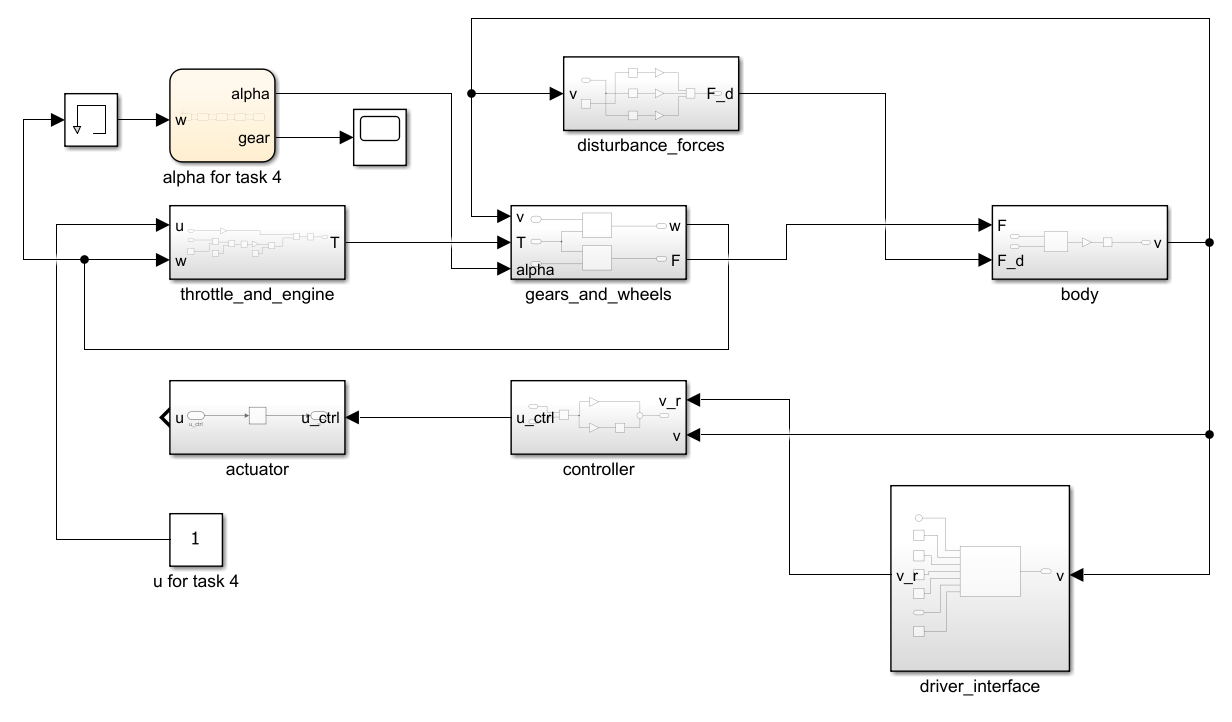
\includegraphics[width=0.9\linewidth]{src/figure10.png}
    \caption{Overall Simulink Structure of Task 4}
    \label{fig:task4_overall}
\end{figure}

\begin{figure}[htbp]
    \centering
    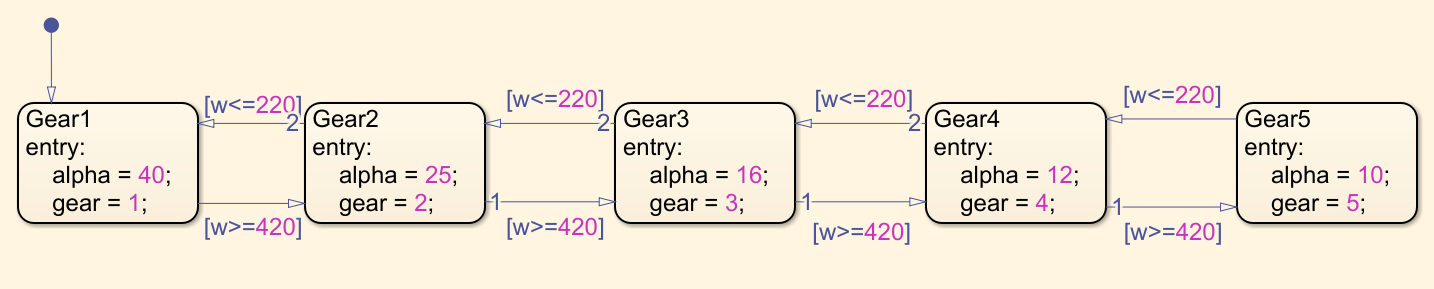
\includegraphics[width=1\linewidth]{src/figure11.png}
    \caption{Stateflow Chart}
    \label{fig:task4_stateflow}
\end{figure}

\begin{figure}[htbp]
    \centering
    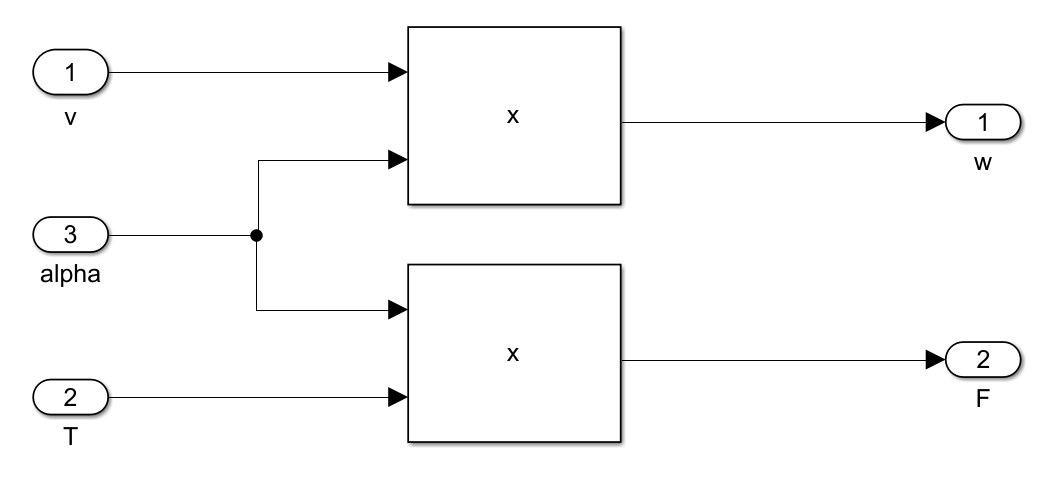
\includegraphics[width=0.8\linewidth]{src/figure12.png}
    \caption{Structure of Subsystem \textit{Gears and wheels} in Task 4}
    \label{fig:task4_gears_and_wheels}
\end{figure}

\subsection{Stateflow Chart Design}

\subsubsection{Memory Block}

In the top-level architecture (see Figure \ref{fig:task4_overall}), there is a memory block before the stateflow chart. This is because an algebraic loop of $\omega$ exists in the top-level architecture, which will be refused by Simulink. To break the algebraic loop, a memory block is inserted upstream of the stateflow input. By introducing a single time-step delay, the Stateflow block receives the previous step's state instead of the current state, which eliminates the algebraic loop.

\subsubsection{Transition Conditions}

If the car shift the gear from $i$ to $j$, since instantaneous speed remains unchanged during the transition, according to equation \ref{eq:w=av}, the new engine rotation speed is:

\begin{equation}
    \omega_j = \frac{\alpha_j}{\alpha_i}\omega_i
    \label{eq:new_omega}
\end{equation}

Define the parameter $p^j_i=\frac{\alpha_j}{\alpha_i}$, then the value of $p^j_i$ is shown as table \ref{tab:p_shift}.

\begin{table}[htbp]
    \centering
    \begin{tabular}{c|cccc|cccc}
    \hline
        Gear & 1-2 & 2-3 & 3-4 & 4-5 & 5-4 & 4-3 & 3-2 & 2-1 \\ 
    \hline
        $p^j_i$ & 0.625 & 0.64 & 0.75 & 0.8333 & 1.6 & 1.5625 & 1.3333 & 1.2 \\
    \hline
    \end{tabular}
    \caption{Value of parameter $p^j_i$ when shifting gear}
    \label{tab:p_shift}
\end{table}

Define the engine rotation speed of upshifting as $\omega_{up}$, and downshifting as $\omega_{down}$, which should meet the following conditions preventing from gear oscillation:

\begin{equation}
    \begin{cases}
    \omega_{down} \le \min(p^j_i) \cdot \omega_{up}, & i < j \\
    \omega_{up} \ge \max(p^j_i) \cdot \omega_{down}, & i > j \\
    \omega_{down} \ge 0 \\
    \omega_{up} \ge \omega_m
    \end{cases}
    \label{eq:task4_w}
\end{equation}

To ensure that the engine's performance is utilized to the fullest extent, $\omega_{up}$ should be greater but closer to $\omega_m$ as much as possible. Since $\omega_m = 450 rad/s$, we define $\omega_{up} = 460 rad/s$, then $\omega_{down}$ should be less than 287.5 rad/s and bigger than 0. We take the value of $\omega_{down}$ as 220 rad/s.

\subsection{Simulation Conditions}

\textbf{The initial condition of the integrator:}

- In subsystem \textit{Body}: 0, since the initial velocity of the vehicle is 0.

- In subsystem \textit{Controller}: any value, since the top-level system is an open-loop system.

\textbf{Initial gear:} 1, and at the same time $\alpha = \alpha_1 = 40$.

Table \ref{tab:task4_simcondition} shows the initial simulation conditions in task 4.

\begin{table}[htbp]
    \centering
    \begin{tabular}{cccc}
       \hline
       Parameter & Variable & Value & Unit \\
       \hline
       Gear & / & 1 & / \\
       Transmission ratio & $\alpha_n (\alpha_1)$ & 40 & $rad/m$\\
       Throttle position & $u$ & 1 & / \\
       Road slope & $\theta$ & 0 & $deg$ \\ 
       Initial speed (integrator initial condition) & $v(0)$ & 0 & m/s \\
       Goal speed & $v_r$ & any & m/s \\
       Proportion Coefficient & $k_p$ & any & / \\
       Integral Coefficient & $k_i$ & any & / \\
       Output & $v$ & / & m/s \\
    \hline
    \end{tabular}
    \caption{Initial Simulation Conditions in Task 4}
    \label{tab:task4_simcondition}
\end{table}

\subsection{Simulation results}

Figure \ref{fig:task4_simresult_0_20} and \ref{fig:task4_simresult_0_100} show the simulation results of vehicle speed, engine rotational speed and gear in task 4. The unit of y-axis (speed) has been changed from m/s to km/h.

\begin{figure}[htbp]
    \centering
    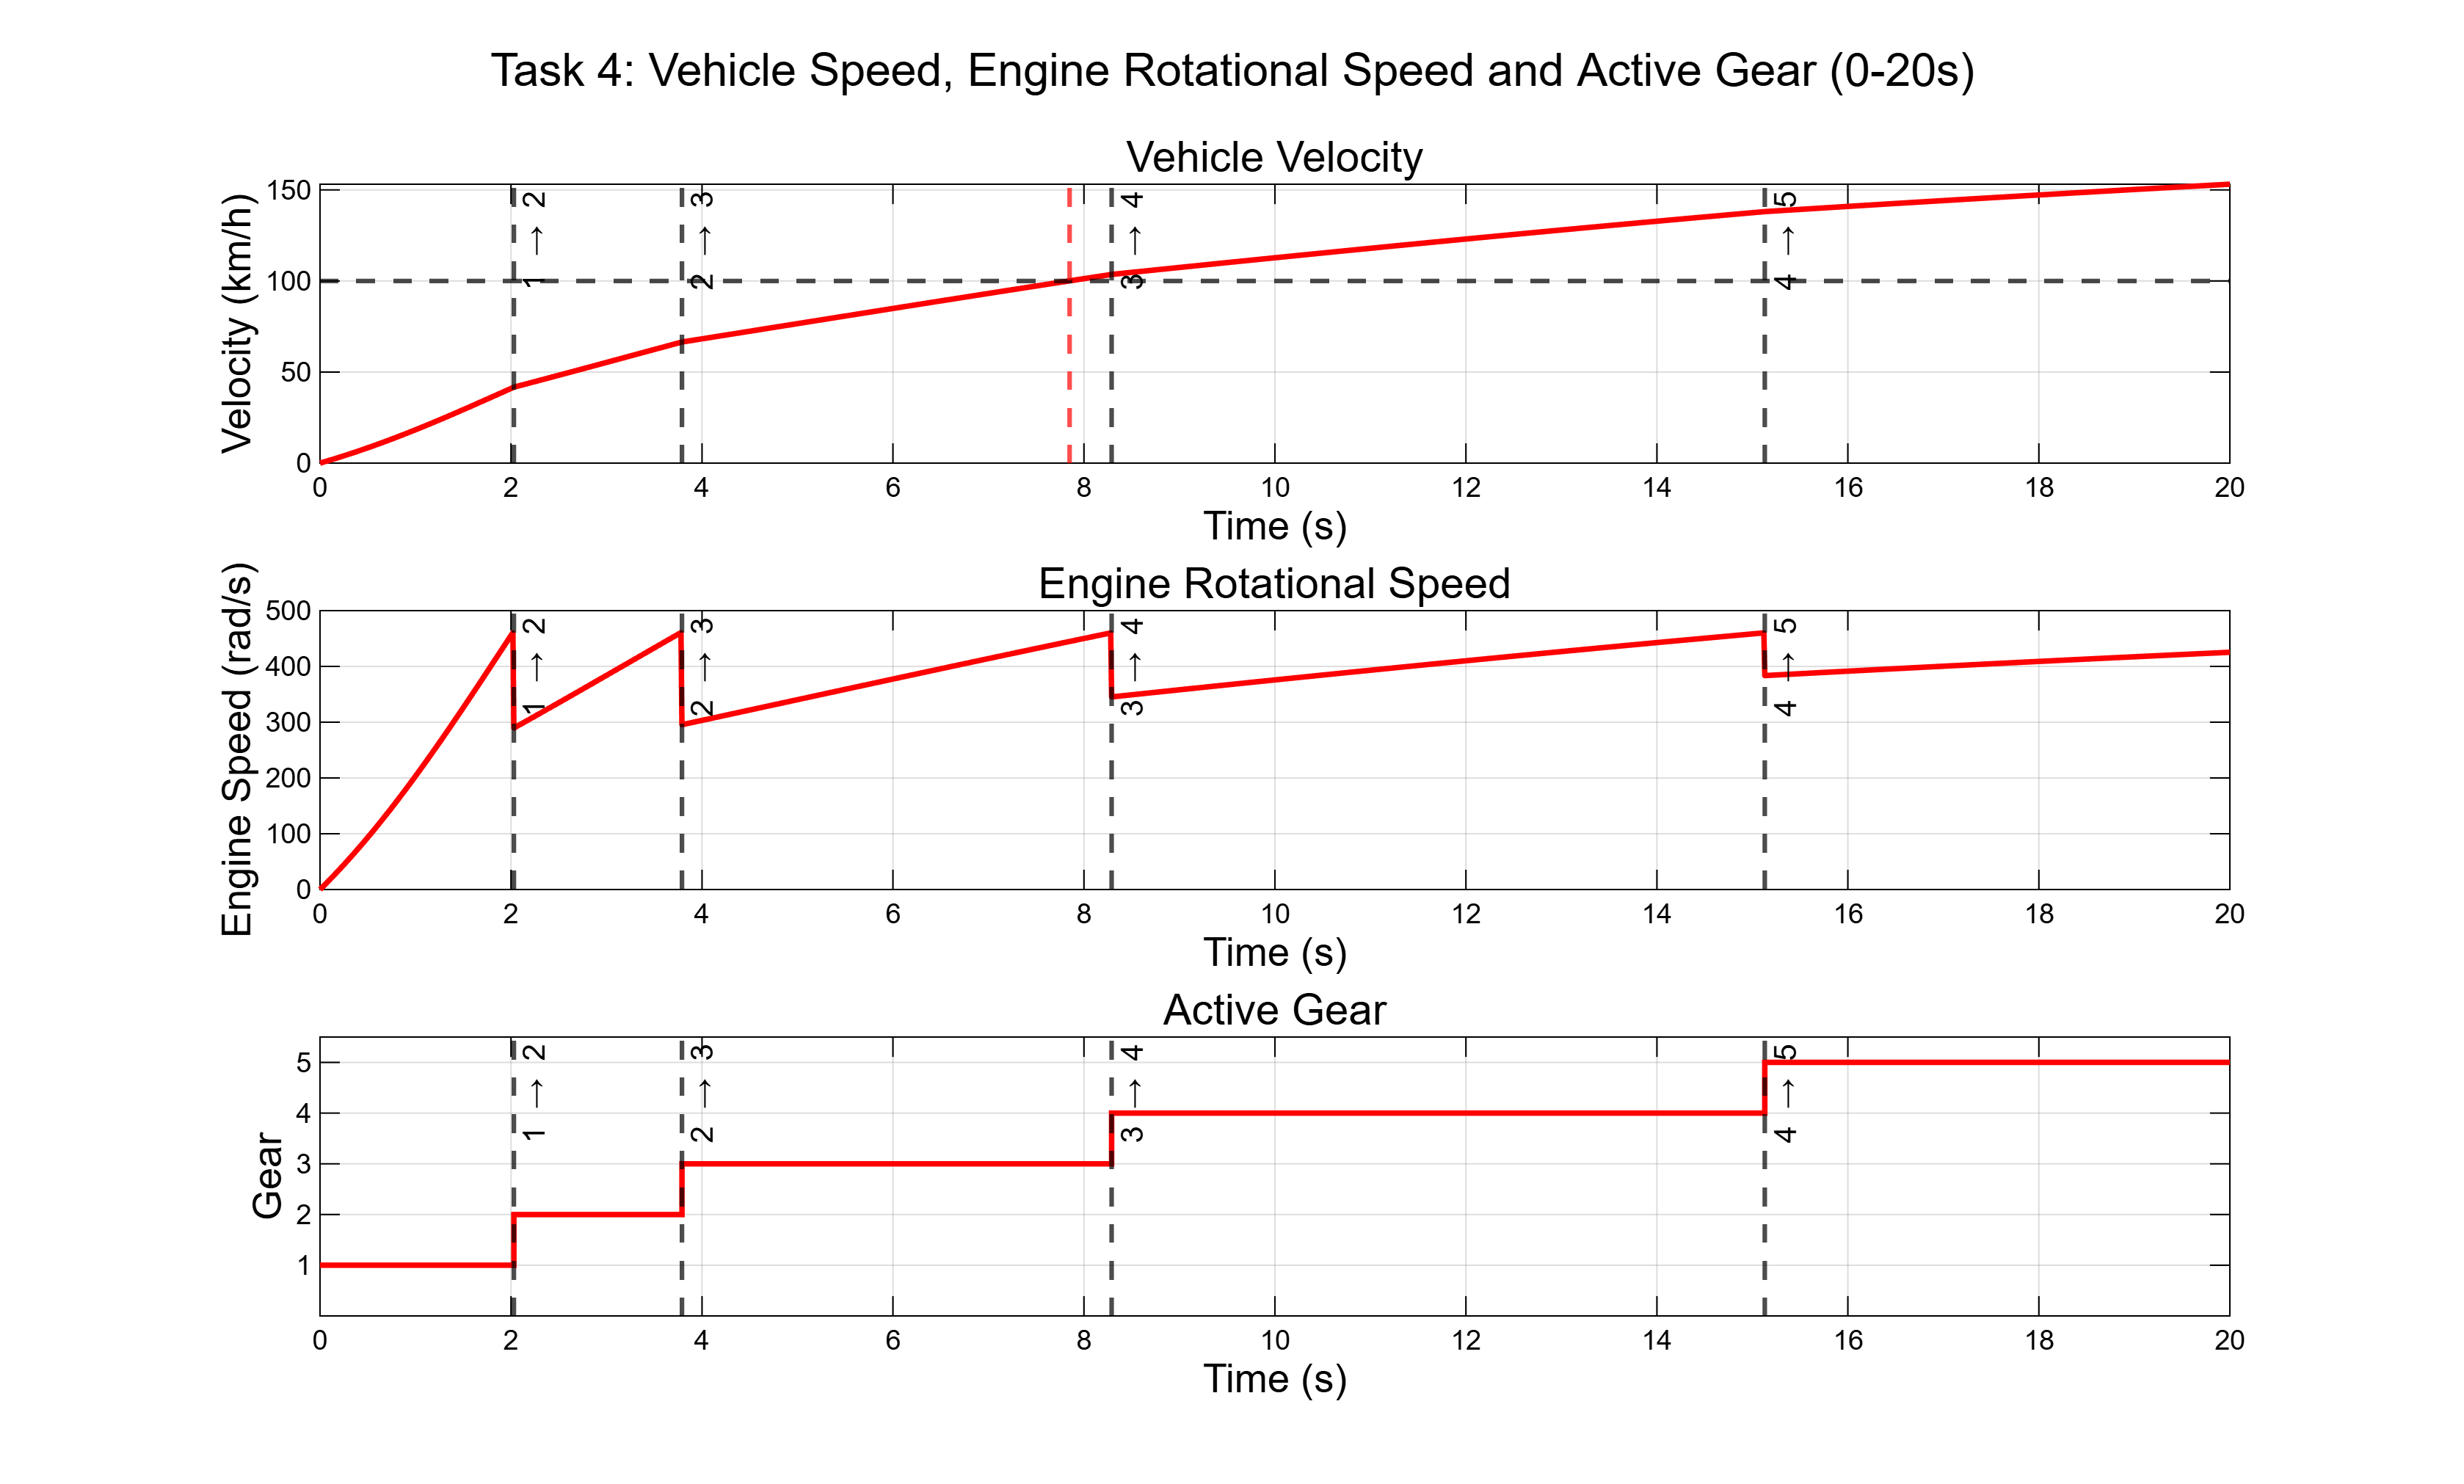
\includegraphics[width=1\linewidth]{src/task4_20s.png}
    \caption{Simulation result of 0 - 20 s of Task 4}
    \label{fig:task4_simresult_0_20}
\end{figure}

\begin{figure}[htbp]
    \centering
    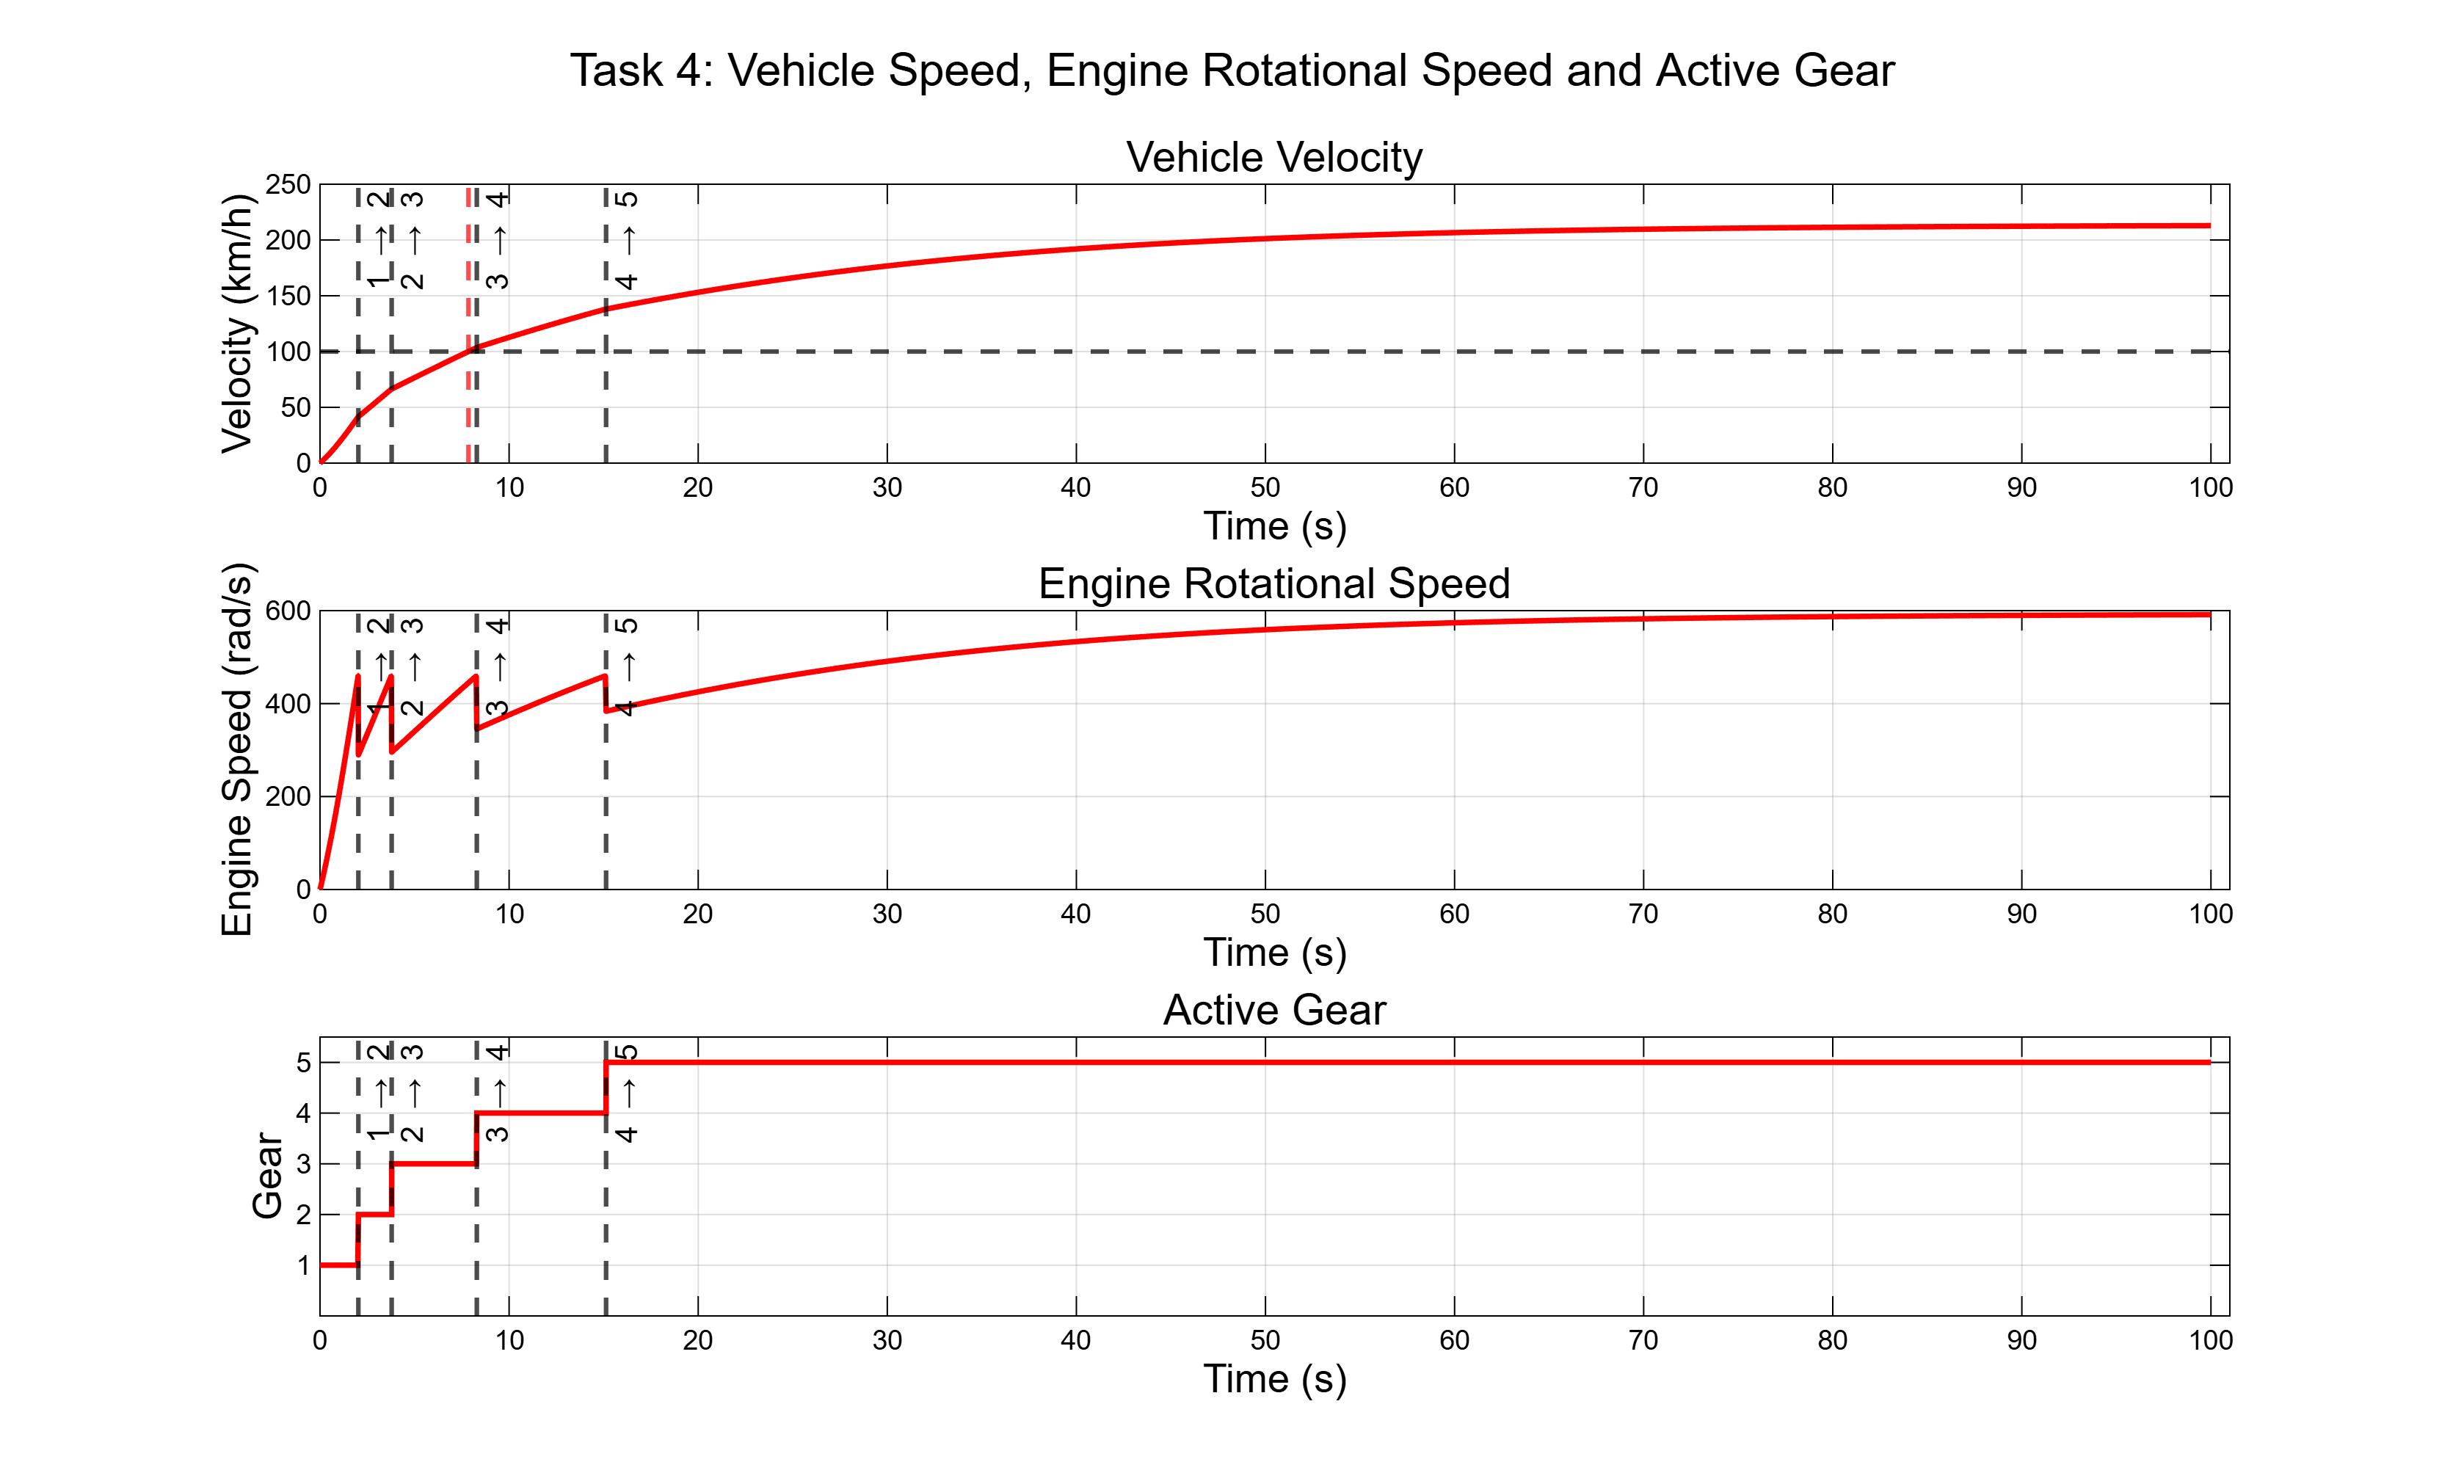
\includegraphics[width=1\linewidth]{src/task4_100s.png}
    \caption{Simulation result of 0 - 100 s of Task 4}
    \label{fig:task4_simresult_0_100}
\end{figure}

According to the raw data and code execution result, the simulation results are in table \ref{tab:task4_simresult}.

\begin{table}[htbp]
    \centering
    \begin{tabular}{cc}
    \hline
        Time of 100 km/h & 7.85 s \\
        Time of gear 1 to 2 & 2.03 s \\
        Time of gear 2 to 3 & 3.79 s \\
        Time of gear 3 to 4 & 8.29 s \\
        Time of gear 4 to 5 & 15.13 s \\
    \hline
    \end{tabular}
    \caption{Simulation Result of Task 4}
    \label{tab:task4_simresult}
\end{table}

When the vehicle reached 100 km/h, the gear level hasn't been fully upgraded, which is 3, not 5.

\section{Other Information}

1. MATLAB version: R2026a.

2. All the data are measured from the raw data by using the "to workspace" block in Simulink. This block will output the exact value of the measured variable and its corresponding time. No data are measured directly from the output image or the scope model from Simulink.

3. Theoretical calculation of $k_p$ and $k_i$ in task 3:

Perform a first-order Taylor expansion on equation \ref{eq:newton_2nd_law_eq1} at the point $(u_0, v_0) = (0, 20)$ of $t=0$:

\begin{equation}
    m\cdot \frac{d\Delta v}{dt} \approx 
    \frac{\partial F}{\partial u}|_{(u_0, v_0)} \cdot \Delta u + 
    \frac{\partial F}{\partial v}|_{(u_0, v_0)} \cdot \Delta v +
    \frac{\partial F_d}{\partial u}|_{(u_0, v_0)} \cdot \Delta u +
    \frac{\partial F_d}{\partial v}|_{(u_0, v_0)} \cdot \Delta v
    \label{eq:taylor1}
\end{equation}

Since $F_d$ is independent to $u$ according to \ref{eq:fraction}, then:

\begin{equation}
    m\cdot \frac{d\Delta v}{dt} \approx 
    \frac{\partial F}{\partial u}|_{(u_0, v_0)} \cdot \Delta u + 
    \frac{\partial F}{\partial v}|_{(u_0, v_0)} \cdot \Delta v +
    \frac{\partial F_d}{\partial v}|_{v_0} \cdot \Delta v = 
    \frac{\partial F}{\partial u}|_{(u_0, v_0)} \cdot \Delta u + 
    (\frac{\partial F}{\partial u}|_{(u_0, v_0)} + \frac{\partial F_d}{\partial v}|_{v_0}) \Delta v
    \label{eq:taylor2}
\end{equation}

Define:

\begin{gather}
    a_0 = \frac{\partial F}{\partial u}|_{(u_0, v_0)} + \frac{\partial F_d}{\partial v}|_{v_0} =
    \rho C_d A v_0 + 2 \alpha_3^2 \beta u_0 T_m \frac{\alpha_3 v_0 - \omega_m}{\omega_m^2}
    \label{wq:a0} \\
    b_0 = \frac{\partial F}{\partial u}|_{(u_0, v_0)} = \alpha_3 T_m [1-\beta(\frac{\alpha_3 v_0}{\omega_m}-1)^2]
    \label{eq:b0}
\end{gather}

Then we get $m\frac{d\Delta v}{dt} + a_0 \Delta v = b_0 \Delta u$. Apply the Laplace transform to both sides of the equation, and we get the transfer function $G(s)$ of $\Delta V(s)$ with respect to $\Delta U(s)$:

\begin{gather}
    sm\Delta V(s) + a_0 \Delta V(s) = b_0 \Delta U(s)
    \label{eq:laplace} \\
    G(s) = \frac{\Delta V(s)}{\Delta U(s)} = \frac{b_0}{ms+a_0} =
    \frac{\frac{b_0}{m}}{s+\frac{a_0}{m}} \approx \frac{2.5888}{s + 0.01915}
    \label{eq:gs}
\end{gather}

Thus, there is a pole point $s = -0.01915 rad/s$ of the vehicle. We need to design a controller with a zero point -0.01915 to eliminate the effect of the pole, which is:

The open-loop transfer function of PI control system:

\begin{equation}
    C(s) = k_p + \frac{k_i}{s} = \frac{1}{s}[k_p(s+\frac{k_i}{k_p})]
\end{equation}

The open-loop transfer function of the whole system:

\begin{equation}
    L(s) = C(s)G(s) = k_p(\frac{s+\frac{k_i}{k_p}}{s})(\frac{\frac{b_0}{m}}{s+\frac{a_0}{m}}) 
\end{equation}

Make a pole-zero cancellation if $\frac{k_i}{k_p} = \frac{a_0}{m}$, then:

\begin{equation}
    L(s) = \frac{k_p \cdot b_0}{m\cdot s}
\end{equation}

The close-loop transfer function of the whole control system is:

\begin{equation}
    T(s) = \frac{L(s)}{1+L(s)} = \frac{\frac{k_p \cdot b_0}{m\cdot s}}{1+\frac{k_p \cdot b_0}{m\cdot s}} = 
    \frac{1}{\tau_{cl}+1}
\end{equation}

where $\tau_{cl} = \frac{m}{k_p \cdot b_0}$. If we define the time constant $\tau_{cl} = 1.5s$, then:

\begin{gather}
    k_p = \frac{m}{b_0 \cdot \tau_{cl}} \approx 0.2575 \\
    k_i = k_p \cdot \frac{a_0}{m} \approx 0.00493
\end{gather}

In task 3, we choose $k_p = 0.24, k_i = 0.0006$.

4. $\omega_m$ is the engine speed of maximum output torque, not the maximum engine rotational speed.

5. All the "to workspace" models have a sampling time of 0.01 s rather the default -1.

\end{document}
